\documentclass[11pt,a4paper]{article}
\usepackage[spanish]{babel}
\usepackage[utf8]{inputenc}
\usepackage[T1]{fontenc}
\usepackage{graphicx}
\usepackage{geometry}
\usepackage{hyperref}
\usepackage{enumitem}
\geometry{margin=2.5cm}

\graphicspath{{graphics/}}

\title{Sistema de Gestión Polimórfica de Sensores para IoT}
\author{Reporte Técnico}
\date{\today}

\begin{document}

\maketitle

\section{Introducción}

El presente documento describe la solución implementada para el caso de estudio de la unidad: un sistema de monitoreo polimórfico que administra sensores heterogéneos (temperatura y presión) empleando listas enlazadas simples sin depender de la STL. El objetivo principal es registrar lecturas, procesarlas con lógica específica por sensor y liberar memoria de forma segura, todo mientras se conserva un único contenedor polimórfico y se habilita la integración con un dispositivo Arduino/ESP32 mediante puerto serial.

\section{Manual Técnico}

\subsection{Diseño General}

\begin{itemize}[leftmargin=1.5em]
    \item \textbf{Jerarquía de Sensores:} La clase abstracta \texttt{SensorBase} define la interfaz común \\ (\texttt{imprimirInfo()}, \texttt{registrarLecturaInteractiva()}, \texttt{registrarLecturaDesdeCadena()} y \texttt{procesarLectura()}). Las clases derivadas \texttt{SensorTemperatura} y \texttt{SensorPresion} implementan la lógica específica para lecturas \texttt{float} e \texttt{int}, respectivamente, incluyendo la eliminación del mínimo (temperatura) y el cálculo de promedio (presión).
    \item \textbf{Contenedor Polimórfico:} \texttt{ListaGeneral} gestiona punteros a \texttt{SensorBase} mediante una lista enlazada manual. Se asegura que cada sensor se inserte solo una vez y al liberar la lista se invocan los destructores correctos gracias al destructor virtual.
    \item \textbf{Listas Genéricas:} Las lecturas internas utilizan \texttt{ListaSensor<T>} y \texttt{Nodo<T>}, plantillas que implementan inserción al final, búsqueda, extracción, cálculo de promedio y regla de los tres (constructor de copia, asignación y destructor). Esto cumple con el requisito de manejar memoria dinámica sin STL.
    \item \textbf{Interacción CLI:} \texttt{AuxiliarCli} centraliza la captura validada de datos y el formateo de logs coloreados (\texttt{STATUS}, \texttt{WARNING}, \texttt{SUCCESS}). Los mensajes \texttt{ERROR} se reservan para cierres críticos, como se estipuló.
\end{itemize}

\subsection{Flujo de Ejecución}

El módulo principal (\texttt{src/main.cpp}) ofrece un menú que permite:
\begin{enumerate}[leftmargin=1.5em]
    \item Crear sensores de temperatura o presión, solicitando un identificador textual.
    \item Registrar lecturas ya sea manualmente o mediante una línea \texttt{ID,valor} proveniente del puerto serial.
    \item Procesar polimórficamente todas las lecturas registradas.
    \item Liberar la memoria de manera controlada antes de finalizar.
\end{enumerate}

La compatibilidad con Arduino/ESP32 se valida con el sketch \texttt{arduino/SerialEmitter.ino}, que emite periódicamente lecturas en el formato requerido. El programa principal parsea estas cadenas y delega el registro a cada sensor.

\subsection{Componentes Relevantes}

\begin{itemize}[leftmargin=1.5em]
    \item \textbf{CMake:} El archivo \texttt{CMakeLists.txt} compila el binario \texttt{gestion\_sensores}, incluyendo el directorio \texttt{include/}.
    \item \textbf{Doxygen:} La configuración \texttt{Doxyfile} genera la documentación HTML dentro de \texttt{docs/html/}, con comentarios breves en cada archivo y método.
    \item \textbf{Simulación Serial:} El proyecto añade la carpeta \texttt{arduino/} con el sketch que produce lecturas de ejemplo para integrar el día de la demostración.
    \item \textbf{Manejo de Memoria:} Todos los destructores informan su actividad con \texttt{AuxiliarCli}, evidenciando la liberación de nodos internos y evitando fugas.
\end{itemize}

\section{Evidencia de Funcionamiento}

\begin{figure}[h]
    \centering
    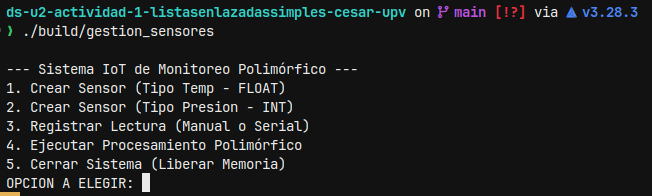
\includegraphics[width=0.8\linewidth]{alIniciarPrograma.png}
    \caption{Estado inicial del menú principal al ejecutar el binario.}
    \label{fig:inicio}
\end{figure}

\begin{figure}[h]
    \centering
    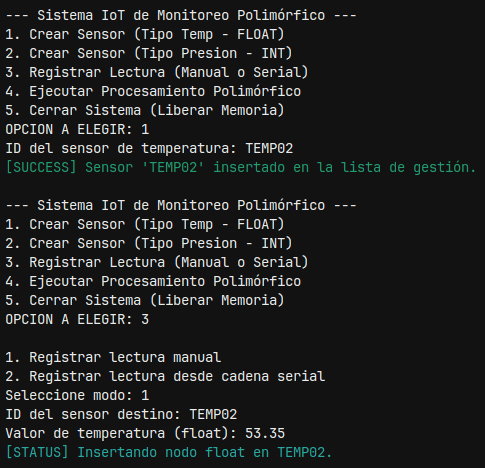
\includegraphics[width=0.8\linewidth]{crearSensorYLectura.png}
    \caption{Creación de un sensor y registro de lecturas manuales utilizando \texttt{AuxiliarCli}.}
    \label{fig:crear}
\end{figure}

\begin{figure}[h]
    \centering
    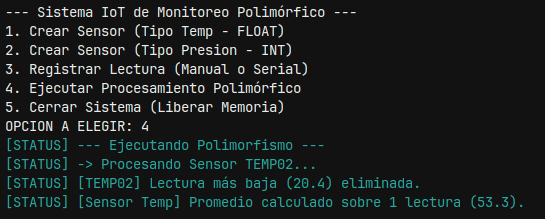
\includegraphics[width=0.8\linewidth]{ejecutarProcesamientoPolimorfico.png}
    \caption{Ejecución del procesamiento polimórfico con la lógica de cada derivada.}
    \label{fig:procesar}
\end{figure}

\begin{figure}[h]
    \centering
    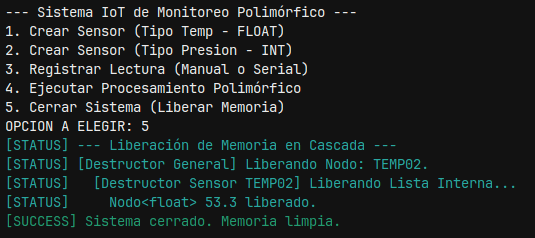
\includegraphics[width=0.8\linewidth]{salirDelPrograma.png}
    \caption{Liberación ordenada de memoria al cerrar el sistema.}
    \label{fig:salir}
\end{figure}

\clearpage

\section{Conclusiones}

La solución cumple con los requerimientos funcionales y no funcionales descritos en el \texttt{README.md}:
\begin{itemize}[leftmargin=1.5em]
    \item Uso estricto de listas enlazadas manuales y plantillas para gestionar lecturas.
    \item Jerarquía polimórfica con métodos virtuales puros y destructores seguros.
    \item Integración con entradas seriales y logs uniformes mediante \texttt{AuxiliarCli}.
    \item Documentación automatizada, estructura modular (\texttt{include/}, \texttt{src/}) y soporte CMake.
\end{itemize}

Se recomienda, como trabajo futuro, añadir pruebas automatizadas y ampliar la jerarquía con nuevos tipos de sensores para demostrar extensibilidad.

\end{document}
